\section{Outlook and guidance for future separators}

\subsection{Recoil separators planned and under construction}

At the time of writing, there are a handful of recoil separators being constructed or in the conceptual or design phase at laboratories worldwide. It is not the intention of the authors to summarize all of these proposals, as some of these may evolve in design or modify their scientific focus. However there are a couple of developments worth mentioning here, specifically projects that are aimed at astrophysics and are under detailed design or construction now. 

St. George (Strong Gradient Electromagnetic Online Recoil separator for capture Gamma-ray Experiments) \cite{cou08} is a recoil separator under construction at the Institute for Structure and Nuclear Astrophysics at the University of Notre Dame. The design is optimized for the study of astrophysical low energy ($\alpha,\gamma$) reactions for up to A=40 beam mass. The beams will be provided by the new 5MV accelerator at the laboratory. The separator has design acceptance values of $\pm$40 mrad in angle and $\pm$7.5\% in energy. It is built in a configuration providing selection of a single charge state via magnetic analysis, before mass separation is performed in a Wien filter (see figure \ref{fig:stgeorge}), with a final resolving power of $m/\Delta m=100$. It is designed to have high a beam suppression factor of $\ge10^{15}$. In particular the Wien filter element of this separator is specially optimized to improve the filtering efficiency, achieved by minimizing the magnetic dipole component fringe fields and by incorporating specially-shaped electrodes so that the electric fringe fields closely follow the magnetic ones. 

The Separator for Capture Reactions (SECAR) is a recoil separator design destined to be a flagship experiment at the Facility for Rare Isotope Beams (FRIB)  at the National Superconducting Cyclotron Laboratory (NSCL) at Michigan State University. The present design is based on the St. George separator, but using an additional Wien filter \cite{ber10}. The separator will operate using reaccelerated radioactive ion beams produced by fragmentation at FRIB and prepared using a gas stopper system. The scientific purpose of this experiment is to continue the study of proton- and alpha- induced radiative capture reactions for explosive nucleosynthesis and represents an important part of the US nuclear physics community's long range plan. The JENSA jet gas target mentioned in section \ref{gas} \cite{chi13} is planned for use with the SECAR separator. 
\begin{figure*}
\begin{center}
\resizebox{1.8\columnwidth}{!}{
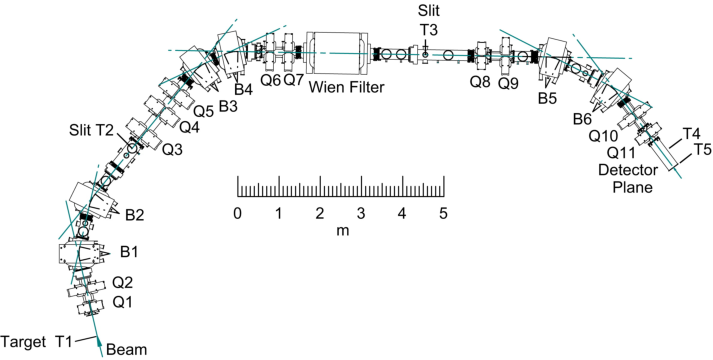
\includegraphics{stgeorge}
}
%\vspace{5cm}       % Give the correct figure height in cm
\caption{Schematic of the St. George recoil separator at the Institute for Nuclear Structure and Astrophysics, Notre Dame University (currently under construction). Taken from \cite{cou08}.}
\label{fig:stgeorge}
\end{center}
\end{figure*}

\subsection{Suggested avenues of technical development} 

With the pioneering measurements made of radiative capture in inverse kinematics over the last few decades, much has been learned and many techniques have been refined. With new recoil separators planned at radioactive beam or `rare isotope' facilities around the world, the proponents have a variety of solutions and methods at their disposal to enable very difficult measurements to take place. One factor that should be considered in the building of recoils separators is versatility. A separator like DRAGON, for example, was built to study lower mass capture reactions with very intense radioactive beams of large emittance, and thus had to have extremely good beam suppression, but at the expense of geometric acceptance. This limited the number of feasible reactions somewhat (or rather simply required extensive simulation to determine efficiencies with a resulting increase in systematic uncertainties). However it has been shown that the separator, with minor modifications, could be used successfully for a program in high mass radiative reactions ($A>70$). Other separators may similarly find new avenues of performance that are beyond what was planned in the design stage. There are several areas in which the authors might suggest, based on their knowledge of past performance of recoil separators, that improvements can be made to ensure versatility.

\subsubsection{Acceptance}

The geometric acceptance, in particular, of a separator is a parameter of vital importance since it can severely limit the range of reactions that can be measured. For small acceptance separators, performing reactions which have a cone angle larger than the acceptance requires extensive simulation, which in principle is not a problem if the angular distribution of the recoils is known (i.e. the $\gamma$-ray cascade transitions and angular distributions). However this does require that any apertures be aligned to very high precision. The nature of differential pumping schemes is such that many apertures are required, leading to the possibility of multiple misalignments. It is recommended that even if a large acceptance is planned for a separator, the limiting apertures should be adjustable and able to be aligned to high precision. Such alignment abilities should also apply to ion-optical elements, using modern, non-invasive (don't have to break vacuum) methods of surveying such as laser-based trackers.\\
In addition, since acceptance is effectively a function of target length in most recoil separators, a versatile target that can house a gas jet, shortened or extended target could be considered, as well as the ability to replace limiting apertures with larger or smaller ones for specific experiments. \\
Vacuum boxes in magnetic dipoles or quadrupole bores can be constraining sources of geometric acceptance that are difficult to change if an `acceptance upgrade' is desired, so all reasonable attempts to maximize these dimensions should be made.

\subsubsection{Rigidity}

Rigidity is often a defining parameter of a recoil separator as magnetic and electrostatic elements come with maximum operable field strengths. However, upgrading a separator to operate beyond its maximum design rigidity is only a technical matter. Magnetic elements are limited usually only by the capacity of the corresponding power supplies, the ability to cool the supplies and the magnets, and the ability to measure the magnetic fields precisely enough for your purposes over a wide enough energy range. 

For example, a magnetic dipole in a MEME design like DRAGON is essential for determination of the beam energy, and thus requires precise $\vec{B}$ measurement, usually using a nuclear magnetic resonance probe.  Such probes tend to have certain operable ranges within a minimum and maximum field strength. For a typical recoil separator interested in low energy reactions typical of stellar and nova scenarios, a single probe may be able to span a range of around 0.1-0.6 tesla, enough for a wide variety of available light-mass recoil charge states and momenta. However, for high mass reactions it gets more difficult to equilibrate in very high charge states, even with charge state boosting devices installed after the gas target. This means the rigidity requirements become more stringent, and it would be beneficial to be able to operate with much higher fields. In that case, consideration could be given to being able to switch between two installed NMR probes for operation in low and high field ranges, and to provide the capability of a cooling boost for the power supplies when operating in the high field region.   

In MEME designs the electric field becomes the limit as one goes to higher charge states as was seen in figure \ref{fig:rigidity}. In that case it is the conditioning ability and the power supply capability that limits going to higher field strengths. Although the electric dipoles at the DRAGON facility have only been able to go as high as $\pm230$ kV because of conditioning issues, new designs like the EMMA dipoles will be able to reach as much as $\pm300$ kV over a 12.5 cm gap \cite{dav05} leading to a maximum field gradient of 5 MV/m compared to to DRAGON's 4.6 MV/m, and a maximum rigidity of 25 MV due to the larger bending radius. Consideration should be given in separator design to the advantages/disadvantages of larger radii/rigidity electric devices, and other more logistical requirements such as the available floor space in an experimental area may come into play when doing this, an issue that also affects Wien filters due to the need for internal or external power supplies. 
 
\subsubsection{Operation}

Operation of a recoil separator includes many aspects such as vacuum cycling, beam tuning and alignment, ion-optical element scaling, diagnostics and data acquisition. These aspects can be of more importance than perhaps realized, since they contribute to the overall length, stability and difficulty of an experiment. 

On the vacuum side, a separator consisting of many sections will require extensive pump down time. It is desirable to split the separator into as many sections as possible however, since particular ones will require access for the maintenance/adjustment of diagnostic devices or other equipment such as foils. Elements such as electric dipoles benefit from staying under vacuum permanently, so appropriate pumps should be chosen that have relatively low wear, such as sputter ion pumps for the long periods of non-use, with additional pumping implemented when operational (e.g. turbomolecular pumps or cryogenic pumps). Although the requirements of the separator vacuum are not as stringent as a UHV system, it is advisable that copper seals are used for joints where there is little expectation of an access requirement, since identifying decade-old decomposing o-rings out of a selection of hundreds is a difficult and time consuming task.

For beam tuning, one has to consider that the facility may be using radioactive or stable beams, and thus may run with intensities ranging anywhere from $10^{6}$ s$^{-1}$ to $10^{13}$ s$^{-1}$, the former being the minimum really possible intensity given typical resonant radiative capture cross sections and typical target densities available, for specific beams and energies, the maximum being the typical kind of current to be expected from a low-energy accelerator system with space-charge constraints. For most of this range, Faraday cup measurements, wire scanners and split-plate centering monitors are sufficient in order to tune a beam of given $A/q$ through the separator. However, attention should be given to the high current end since a beam of $\mu$A current level at $1A$ MeV deposits a power on the order of Watts and rising above this level without proper cooling in vacuum can become problematic. Thus Faraday cups should be built with the ability to cool, similar to as in any high-intensity accelerator facility. Faraday cups require extremely sensitive current amplifiers for the low intensity end of this scale. Picoammeter units are in existence which can provide sufficient resolution ($\sim$20 fA) for tuning and normalization at even below the $10^{5}$ s$^{-1}$ level. However such units are perhaps currently too expensive to populate an entire recoil separator, and are difficult to use in the often complex environment of an experimental hall. Having one Faraday cup that can be instrumented with this can provide however, an anchor point for other means of measurement to be referenced to. 

A less expensive way to measure low beam intensities is to use a device such as an electron multiplier (channeltron). However, these tend to saturate above $10^{6}$ s$^{-1}$, making that difficult $10^{6}-10^{7}$ s$^{-1}$ region stay inaccessible. However, recent developments at the DRAGON facility \cite{chr14} have been made to instrument 1 cm $\times$ 1 cm silicon photodiodes (PDs) that can be placed at the separator focal planes to be used as beam tuning guides. The idea being that a radioactive beam of a little less than $10^{7}$ s$^{-1}$, too low to be reliably tuned with regular Faraday cup systems, can be attenuated at the source (after referencing the current to a high-sensitivity ammeter) to the $10^{6}$ s$^{-1}$ level or lower, and the beam tuned using the PD response at the focal points. PDs from a specific manufacturer have shown a robust linear response to beam intensities of this range, as well as providing energy information, and are likely to become extremely useful diagnostic devices in the separator operation.  

Once beam tuning has been achieved, a reliable scaling algorithm is required to switch to recoil detection mode. It is useful here to have stability monitoring algorithms that can check for drift of field strengths or voltages during long runs. In addition, with extensive switching between charge states a scaling algorithm can cause a tune to degrade due to hysteresis of magnetic elements, therefore care should be taken to retune before any data acquisition period. Beam stability is always an issue during these experiments, particularly when delivered by a charge state bred by a stripper foil, as may be required in an ISOL facility that initially delivers singly-charged ions. Such foils degrade over time and cause shifts in beam energy that will cause the beam position or angle to drift at the target position. One suggestion to monitor this drift is that if a charge-dispersive device is present, such as a magnetic dipole, that the unused beam charge states can be intercepted on a position-sensitive segmented strip of conductor in the dispersive plane of the magnet where sensitivity to small variations in momentum is high. This method decouples from any variation in total beam intensity, such as would be seen by a gas target scattering detector for example.

For data acquisition considerations, much work has been done on systems requiring coincidences between events at the target region and focal plane of spectrometers (in our case prompt $\gamma$-ray detection at the target). For example the Gamma Recoil Electron Alpha Tagging (GREAT) spectrometer design at the recoil separator RITU, Jyv\"{a}skyl\"{a} \cite{pag03} employs a triggerless `total data readout' system reliant on synchronized VME `metronome' modules \cite{laz01}. It was in this spirit that the DRAGON group recently developed a new DAQ system based on separate free-running computers for the prompt $\gamma$-ray detection and for the recoil detection, synchronized using TRIUMF in-house built clock modules, with time-stamping of events and coincidence reconstruction on-board the processors using software \cite{chr14b}. Such systems have the advantage of not having the dead-time of one side locked to the other which can be crucial if using RIB where the rate in the $\gamma$-ray detectors might be extremely high. 

\subsubsection{Detection}

For the detection of recoils, the use of an MCP-based local time-of-flight system is extremely useful in all situations. One area of development that has been crucial to this is the ability to suspend large-area carbon foils over fine mesh so that the transmission efficiency is high, and so that the TOF system does not suffer from recoil losses due to large reaction cone angle or accidental mistunes at the end of the separator. Thin diamond-like carbon (DLC) foils of down to 5 $\mu$g/cm$^2$ have successfully been used over an area of 7 cm diameter, such as in the DRAGON facility. This is possible because of the uniformity,  smoothness, and high transmission of the electro-formed mesh used with them. However, these foils are extremely difficult to float using traditional methods, which thus tend to have a low success rate, leading to high costs and overhead in training of personnel. A suggested avenue of development would be a more successful method of layering such a thin foil over a supporting mesh. 

As mentioned in previous sections, high success has been achieved using ionization chambers and double-sided silicon strip detectors. However it is perhaps beneficial to consider a hybrid of both, whereby a large area DSSSD is combined with a one- or two-anode gas ionization region, enclosed by a thin window of large area, perhaps supported using the same type of electro-formed mesh as for the aforementioned TOF system.  Such a system would have the advantage of the more reliable operation, position sensitivity and better energy resolution of the DSSSD, with the energy loss information of gas ionization. DSSSDs of modern type are routinely used in other gas systems with pressures of several torr, and function satisfactorily in typical ionization media such as isobutane. Such a system is under consideration for use at the DRAGON facility. 

For $\gamma$-ray detection, the use of high-efficiency materials such as BGO and NaI has been important. However, there are clear benefits to moving towards a medium with better timing properties, or better energy resolution, or both. The benefits of high efficiency clearly outweigh the benefits of high energy resolution for $\gamma$ rays in these kind of measurements, however there may be particular cases whereby branching ratio determination capability might be important. With the faster timing achieved by going to more modern high-efficiency scintillation materials such as LaBr$_3$, other possibilities become available. For example, timing between recoil-coincident $\gamma$ rays and the accelerator beam bunch arrival time, can give precise and robust information on the reaction position in an extended gas target. This method does not rely on the geometrical distribution/efficiency of the detector array {\em per se}, such as the `$\gamma$-ray hit pattern' method, and does not suffer from the same statistical limitations. In addition, for cascade $\gamma$ rays, LaBr$_3$ has been demonstrated to show $\gamma-\gamma$ coincidence timing resolution capabilities enabling identification of some branches where energy resolution might be lacking to do so. The main barrier to such methods is the high cost of LaBr$_3$ compared to BGO. It is hoped that with future innovation the costs will come down and such arrays might be a staple of future recoil separators. 

\subsubsection{Simulation}

At some level, every recoil separator will rely on computer simulation for some class of reaction, for example those where full recoil angular acceptance is not achieved. Several software suites are available that can do the job of simulation of particle tracing through electromagnetic fields and interaction with materials. For example the \texttt{LISE++} code \cite{lise++} is a useful tool that can effectively track particles produced through fusion-evaporation reactions through magnetic and electric fields, and contains other tools such as energy-loss calculation etc. However, perhaps the most versatile software tool that could be used for simulation of an entire separator including all reaction event generation, particle transport and tracking, as well as interaction with detectors, is the \texttt{GEANT} family of codes. The \texttt{GEANT3} \cite{geant3} simulation of the DRAGON separator with full tracking through the ion optical elements has been implemented, based on \texttt{RAYTRACE} input files. However it is the ability to also have a custom designed radiative capture event generator inside this that makes it really powerful: reactions can proceed through broad or narrow resonances, or by direct capture, and can decay through preprogrammed $\gamma$ transitions with user-defined branchings and angular distributions. Future recoil separator simulations could combine this type with the benefits of the \texttt{GEANT4} extension \texttt{G4Beamline} \cite{geant4}. 

\section{Acknowledgments}
The authors would like to thank D.A. Hutcheon for contributions to the manuscript. Thanks also to B. Davids, G. Christian and A.N. Other for useful comments and suggestions. \\
The TRIUMF author was funded through the Natural Sciences and Engineering Research Council (NSERC) of Canada. The Colorado School of Mines authors were funded through the US Department of Energy grant DE-FG02-93ER40789. 


